\documentclass[conference]{IEEEtran}
\usepackage{amsmath}
\usepackage{newtxtext,newtxmath}
\usepackage{algorithmic}
\usepackage{graphicx}
\usepackage{textcomp}
\usepackage{xcolor}
\usepackage{booktabs}
\usepackage{tabularx}
\usepackage{cite}
\usepackage{float}
\usepackage{graphicx}
\usepackage{hyperref}
\hypersetup{
	hidelinks,
	colorlinks=true,
	linkcolor=black,
	citecolor=black,
	filecolor=black,
	urlcolor=black
}
\usepackage{tikz}
\usetikzlibrary{positioning, arrows.meta, shapes.geometric}
\usetikzlibrary{shapes, positioning, arrows.meta}

\setlength{\parindent}{0pt}

\def\BibTeX{{\rm B\kern-.05em{\sc i\kern-.025em b}\kern-.08em
		T\kern-.1667em\lower.7ex\hbox{E}\kern-.125emX}}



\begin{document}
	
	\title{A Weather-Aware Explainable Machine Learning Framework for Dairy Cattle Milk Yield Prediction}
	
	\maketitle	
	\setlength{\parskip}{0pt}
	\begin{abstract}
		Prediction of the milk yield is a obvious problem in the field of precision dairy farming, where both the environmental and climatic conditions equally affect production performance. Traditional approaches often ignore weather variability factor or provide a little or limited interpretation, reducing their usage in real-world farm decision systems. This paper proposes a weather factor included machine learning framework for obtaining most accurate milk yield prediction, designed strictly around two main research objectives. First, we develop a weather factor included feature engineering framework that adds ambient micro-climatic conditions, designed through real time Open-Meteo API parameters and Gaussian perturbations, with a standard physiological indicator such as the Temperature-Humidity Index (THI). Second, we build an explainable machine learning framework using SHAP (SHapley Additive Explanations) for feature attribution, along with efficient statistical validations (5-fold cross-validation and Wilcoxon signed-rank tests), automated health alerts, and sire genetics evaluations. On a dataset of 3,000 cattle records, five regression models were evaluated under 5-fold cross-validation and an 80:20 hold-out split. Linear Regression achieved the lowest hold-out test MAE ($2.038$~L/day, MAPE~$9.88\%$, $R^2~0.184$) and cross-validation MAE ($2.013 \pm 0.051$~L/day), while XGBoost delivered robust non-linear predictions ($2.076 \pm 0.032$~L/day CV MAE). The low $R^2$ across all models reflects variance attributable to unmeasured biological factors and the use of synthetically assigned weather—a declared limitation of this dataset—rather than model inadequacy. Pairwise Wilcoxon signed-rank tests found no statistically significant performance differences between the top four models, consistent with the methodological constraint that $n=5$ folds yields a minimum attainable two-sided $p$-value of $0.0625$.
	\end{abstract}
	
	\begin{IEEEkeywords}
		Dairy farming, milk yield prediction, explainable AI, weather analytics, feature engineering, precision livestock farming.
	\end{IEEEkeywords}
	
	\section{Introduction}
	Dairy farming productivity system represents an important part of the global agriculture and food security. But, daily milk production is highly sensitive to climatic changes and variations. Change of ambient temperature and humidity cause physiological heat stress in cattle, compromising metabolic function and leading to significant declines in milk yield. Environmental heat stress is a major factor influencing the health and productivity of dairy cattle. It develops when a cow absorbs or generates more heat than it can release into its surroundings. High ambient temperatures—especially when paired with high humidity—interfere with the animal's natural cooling mechanisms, placing a heavy thermal load on its body. When cattle are exposed to these conditions over extended periods, their overall health, feeding patterns, and milk production suffer.
	
	The relationship between environmental heat stress and milk yield is influenced by several factors, including temperature, humidity, lactation stage, feed intake and individual animal characteristics. Therefore, incorporating weather-related parameters and animal-specific characteristics into predictive models can provide a more comprehensive understanding of variations in milk production. This motivates the integration of environmental indicators, particularly THI, into machine learning-based dairy milk-yield prediction frameworks.
	
	To address these gaps, a weather-aware, explainable ML framework for dairy cattle milk yield prediction is presented, with the following specific contributions:
	\begin{enumerate}
		\item A \textbf{weather-aware feature engineering pipeline} that assigns per-animal synthetic microclimate conditions via a seeded Gaussian perturbation model and computes the Temperature-Humidity Index (THI) using the standard Celsius formulation of Mader et al.\ \cite{ref16}.
		\item A \textbf{comparative evaluation} of five regression models (Linear Regression, Decision Tree, Random Forest, SVR, XGBoost) under consistent 5-fold cross-validation and an 80:20 hold-out split.
		\item A \textbf{SHAP-based explainability analysis} identifying biological weight and age-related features as dominant predictors, with weather-derived features providing secondary contributions.
		\item An \textbf{ablation study and noise sensitivity analysis} quantifying the marginal contribution of environmental features and confirming prediction robustness under perturbed weather inputs.
	\end{enumerate}
	
	For building the context for precision agriculture, Internet of Things(IOT) systems, and interpretable machine learning models, a comprehensive review of recent literature is required. Prior work in this domain includes barn microclimate Equivalent Temperature Index forecasting \cite{ref1}, semi-arid dry matter intake modeling \cite{ref2},interpretable SVM-KNN milk yield predictions \cite{ref3},national level milk volume benchmarks \cite{ref4}, group level big data prediction tools and methods \cite{ref5}, meat output regression forecasts using dairy inputs \cite{ref6}, multi-task activity modeling \cite{ref7}, SNP selection for quantitative genetic traits \cite{ref8}, LoRa-based early disease classifiers,wearable edge-AI neckbands \cite{ref9}, crop-weed classification ensembles \cite{ref11}, and non-invasive core temperature monitoring \cite{ref12}.
	
	\setlength{\parskip}{0pt}
	
	Our pipeline fetches real-time weather from the Open-Meteo API, assigns per-animal conditions via Gaussian perturbation, and derives the Temperature-Humidity Index (THI) alongside biological feed ratios. We benchmark five regressors under 5-fold cross-validation, validate model selection with the Wilcoxon signed-rank test, and interpret predictions with TreeSHAP, culminating in a decision-support module with automated alerts and sire genetics rankings.
	
	The remainder of this paper is structured as follows. Section II reviews the literature. Section III gives information about the proposed architecture.Section IV describes the weather factor included feature engineering framework. Section V gives an explanation about the explainable machine learning framework and statistical validation pipeline. Section~V presents the experimental results and model evaluations. Section~VI provides a detailed discussion of the findings, feature ablation, and limitations, and Section~VII concludes the paper.
	
	\section{Literature Review}
	
\begin{table}[!ht]
		\caption{Summary of Related Work in Smart Dairy Farming}
		\label{tab:related_work}
		\centering
		\footnotesize
		\setlength{\tabcolsep}{3pt}
		\begin{tabular}{p{2.0cm} p{2.1cm} p{1.3cm} p{2.6cm}}
			\toprule
			\textbf{Author} & \textbf{\& Method} & \textbf{Dataset} & \textbf{Key Limitation} \\
			\textbf{Year} & & & \\
			\midrule
			Perez Garcia et al. 2025 \cite{ref1} & NeuralProphet ETI & Open-Meteo API & Indoor sensor gaps \\
			Leal et al. 2025 \cite{ref2} & EBETS Fuzzy Model & Semi-arid DMI data & Limited scaling \\
			Srinithi et al. 2025 \cite{ref3} & SVM-KNN + SHAP & TMR feeding data & No dynamic simulation \\
			O'Leary \& Lynch 2022 \cite{ref4} & RF, KNN & Irish national data & Herd-level only \\
			Yan et al. 2015 \cite{ref5} & Big Data Analytics & Supply chain data & Complex design \\
			Prasad 2025 \cite{ref6} & Meat Regression & USDA historical data & Static data \\
			Thangarasu \& Alla 2024 \cite{ref7} & Multi-Task Regularization & Cattle activity data & No yield forecast \\
			Feng et al. 2024 \cite{ref8} & LASSO, SPLS & Canadian Holstein & Needs genomic data \\
			Arafat et al. 2024 \cite{ref9} & IoT + kNN & IoT sensor logs & Hardware dependent \\
			Michelle et al. 2022 \cite{ref10} & Edge-AI Neckband & ESP32 sensor data & Battery constraint \\
			Umamageswaran et al. 2025 \cite{ref11} & CNN + IoT Ensemble & Weed \& sensor data & Needs structured input \\
			Molins et al. 2025 \cite{ref12} & Thermal Image + ML & Vaginal temperature & High sensor cost \\
			\bottomrule
		\end{tabular}
	\end{table}
	Table~\ref{tab:related_work} gives a summary of 12 representative studies covering microclimate forecasting,model explainability,IOT telemetry,and ensemble learning.The occurence of recurring constraint is the result of absence of dynamic, interpretable models which account for localised climatic stress on a per-animal scale
	
	
	\section{Proposed Architecture}
	The Smart Dairy Vision AI framework was developed to study how weather conditions affect dairy cattle productivity and to generate milk-yield predictions that make sense. The complete workflow includes combining datasets creating features that take weather into account predicting milk yield using machine learning analyzing why the model makes predictions and validating the results statistically as shown in Fig.~\ref{fig:system_architecture}
	
	% \begin{figure}[htbp]
		%     \centering
		%     \includegraphics[width=0.95\linewidth]{/Users/sanjana/Downloads/research_1_latex/methodology.png}
		%     \caption{System methodology flowchart detailing Objective 1 (Weather-Aware Feature Engineering Framework) and Objective 2 (Explainable Machine Learning and Validation).}
		%     \label{fig:methodology}
		% \end{figure}
	
	\begin{figure}[htbp]
		\centering
		\resizebox{\columnwidth}{!}{%
			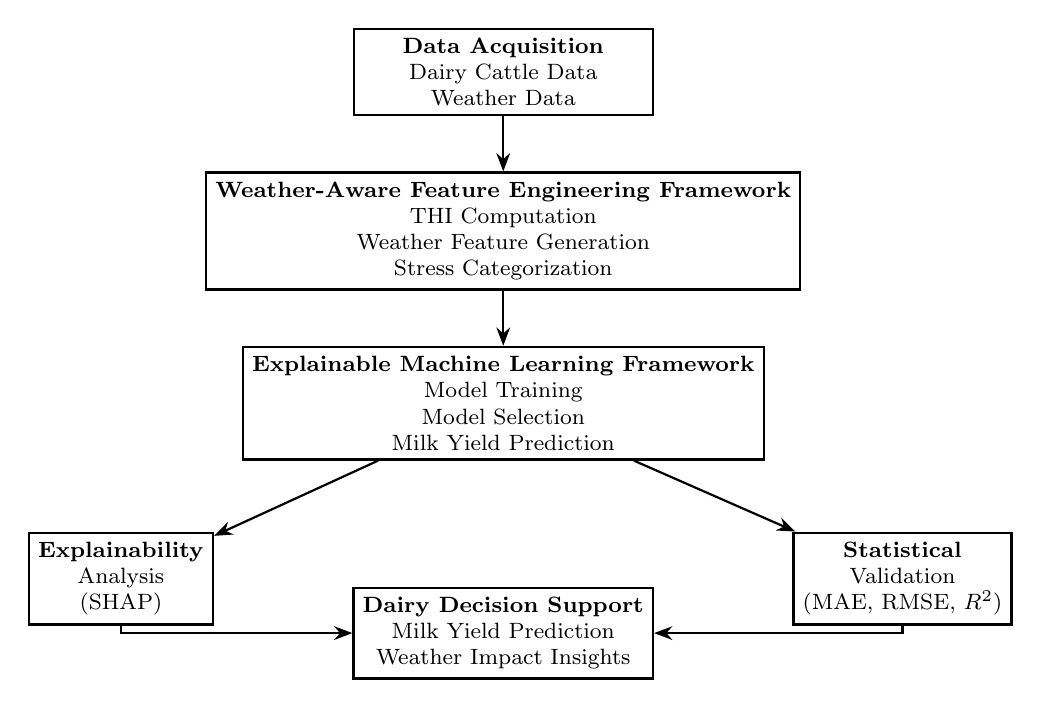
\begin{tikzpicture}[
				node distance=0.7cm,
				block/.style={
					rectangle,
					draw=black,
					thick,
					align=center,
					minimum width=3.8cm,
					minimum height=1.0cm,
					font=\footnotesize
				},
				smallblock/.style={
					rectangle,
					draw=black,
					thick,
					align=center,
					minimum width=1.8cm,
					minimum height=0.9cm,
					font=\footnotesize
				},
				arrow/.style={
					-{Stealth},
					thick
				}
				]
				
				% Block 1
				\node[block] (data) {
					\textbf{Data Acquisition}\\
					Dairy Cattle Data\\
					Weather Data
				};
				
				% Block 2
				\node[block, below=of data] (feature) {
					\textbf{Weather-Aware Feature Engineering Framework}\\
					THI Computation\\
					Weather Feature Generation\\
					Stress Categorization
				};
				
				% Block 3
				\node[block, below=of feature] (ml) {
					\textbf{Explainable Machine Learning Framework}\\
					Model Training\\
					Model Selection\\
					Milk Yield Prediction
				};
				
				% Left branch
				\node[smallblock, below left=0.9cm and 0.35cm of ml] (xai) {
					\textbf{Explainability}\\
					Analysis\\
					(SHAP)
				};
				
				% Right branch
				\node[smallblock, below right=0.9cm and 0.35cm of ml] (stats) {
					\textbf{Statistical}\\
					Validation\\
					(MAE, RMSE, $R^2$)
				};
				
				% Final output
				\node[block, below=1.6cm of ml] (output) {
					\textbf{Dairy Decision Support}\\
					Milk Yield Prediction\\
					Weather Impact Insights
				};
				
				% Arrows
				\draw[arrow] (data) -- (feature);
				\draw[arrow] (feature) -- (ml);
				
				\draw[arrow] (ml) -- (xai);
				\draw[arrow] (ml) -- (stats);
				
				\draw[arrow] (xai) |- (output);
				\draw[arrow] (stats) |- (output);
				
			\end{tikzpicture}%
		}
		
		\caption{System architecture of the proposed weather-aware explainable machine learning framework for dairy cattle analytics and milk-yield prediction.}
		\label{fig:system_architecture}
		
	\end{figure}
	
	\subsection{Data Acquisition and Integration}

	\subsubsection{Dataset Description}
	Two structured tabular datasets, sourced from Kaggle \cite{ref13}, are used in this study.
	Neither dataset contains a date, timestamp, or GPS coordinate column; consequently, no
	date-based weather matching is performed.

	\textbf{Global Cattle Milk Yield Prediction Dataset.}
	This dataset contains 3,000 records and 4 columns.
	\textit{Cattle\_ID} is a unique animal identifier.
	\textit{Feed\_Quantity\_kg} is the daily dry-matter feed intake (kg) and
	serves as the primary nutritional input feature.
	\textit{Lactation\_Stage} records the lactation phase of each animal
	(Early, Mid, or Late); although present in the raw file, this column is not
	included in the model feature set in the current implementation.
	\textit{Milk\_Yield\_L} is the daily milk production in litres and is the
	sole regression target variable ($y$) throughout all experiments.
	Inspection of the raw file confirmed zero missing values and zero exact
	duplicate rows.

	\textbf{Global Cattle Disease Detection Dataset.}
	This dataset contains 3,000 records and 6 columns.
	\textit{Cattle\_ID} is the shared join key.
	\textit{Age\_Months} and \textit{Weight\_kg} are animal-level physiological
	attributes and are used directly as model input features.
	\textit{Breed} and \textit{Body\_Condition} are present in the raw file
	but are not included in the implemented feature set.
	\textit{Disease\_Status} records the health classification of each animal
	(e.g., Healthy, Foot and Mouth); the implementation binary-encodes this
	column into a \textit{health\_status} feature (0 = Healthy, 1 = Diseased)
	that enters the model as a categorical health indicator.
	Inspection confirmed zero missing values and zero exact duplicate rows.

	% ---- Table II: Dataset Characteristics (redesigned) ----
	\begin{table}[!ht]
		\caption{Dataset Characteristics and Final Feature Set}
		\label{tab:dataset_characteristics}
		\centering
		\footnotesize
		\renewcommand{\arraystretch}{1.15}
		\begin{tabularx}{\columnwidth}{@{} l X @{}}
			\toprule
			\textbf{Attribute} & \textbf{Value / Description} \\
			\midrule
			\multicolumn{2}{@{}l}{\textbf{A.~Milk Yield Dataset}} \\
			\quad Records & 3,000 \\
			\quad Raw columns & 4 \\
			\quad Join key & Cattle\_ID \\
			\quad Target & Milk\_Yield\_L (regression target) \\
			\quad Used input & Feed\_Quantity\_kg \\
			\quad Unused & Lactation\_Stage \\
			\midrule
			\multicolumn{2}{@{}l}{\textbf{B.~Disease Detection Dataset}} \\
			\quad Records & 3,000 \\
			\quad Raw columns & 6 \\
			\quad Join key & Cattle\_ID \\
			\quad Used inputs & Age\_Months, Weight\_kg, Disease\_Status \\
			\quad Unused & Breed, Body\_Condition \\
			\quad Encoding & Disease\_Status $\to$ \textit{health\_status} (0\,=\,Healthy; 1\,=\,Diseased) \\
			\midrule
			\multicolumn{2}{@{}l}{\textbf{C.~Final Modelling Dataset}} \\
			\quad Merged records & 3,000 (inner join on Cattle\_ID) \\
			\quad Missing / duplicates & 0 / 0 \\
			\quad Target column & \textit{milk\_output} (L/day) \\
			\quad Model features (12) & \textit{age, weight, health\_status, feed,} \\
			 & \textit{temperature, humidity, thi,} \\
			 & \textit{feed\_weight\_ratio, temp\_humidity,} \\
			 & \textit{thi\_squared, feed\_thi\_interaction,} \\
			 & \textit{age\_weight\_ratio} \\
			\quad Weather / engineered & Synthetically assigned; not original raw columns \\
			\bottomrule
		\end{tabularx}
	\end{table}

	\subsubsection{Dataset Integration}
	Both datasets share an identical, ordered set of 3,000 Cattle\_ID values
	(COW00000–COW02999).
	The implementation in \texttt{data\_loader.py} performs an explicit inner
	join on the \textit{Cattle\_ID} key using \texttt{pandas.merge}, producing
	a merged frame of 3,000 rows and 9 raw columns.
	After renaming (\textit{Age\_Months} $\to$ \textit{age};
	\textit{Weight\_kg} $\to$ \textit{weight};
	\textit{Feed\_Quantity\_kg} $\to$ \textit{feed};
	\textit{Milk\_Yield\_L} $\to$ \textit{milk\_output}),
	standard cleaning is applied: rows containing NaN values in any
	model-relevant column are dropped, and exact duplicate rows are removed.
	Because neither source dataset contains missing values or duplicate rows,
	the merged frame retains all 3,000 records after cleaning.

	\subsubsection{Weather Data Acquisition}
	Because the cattle records carry no timestamps or geographic coordinates,
	date-based weather matching is not feasible.
	The pipeline instead queries the Open-Meteo free API \cite{ref1} at
	run-time to obtain a single \textit{baseline} temperature ($T_{\text{baseline}}$,
	°C) and relative humidity ($RH_{\text{baseline}}$, \%) for a configured
	farm location (default: Bangalore, India; lat~12.97°N, lon~77.59°E).
	If the network request fails, the system falls back to pre-configured
	constants ($T = 28.0$~°C, $RH = 65.0$\%).
	Per-animal ambient conditions are then generated by the Gaussian
	perturbation procedure described in Section~IV, which introduces
	realistic micro-environmental variance across the 3,000 records.
	No weather CSV file is supplied with or read by the pipeline; all
	weather values used in the feature matrix are either API-fetched or
	synthetically generated.

	\textbf{Limitations of Synthetic Weather Data.}
	Per-animal ambient conditions are synthetically generated rather than directly measured or retrieved from archival meteorological records.
	Temperature and relative humidity values are assigned to each record through a parameterised seasonal stochastic model and are independent of the corresponding individual milk yield value.
	Because the source datasets contain neither observation timestamps nor geographic coordinates beyond a single configured location, date-matched or spatially resolved weather retrieval is not feasible.
	Consequently, any association learned by the predictive models between THI-derived features and milk yield reflects patterns introduced by the synthetic generation process, limiting the generalisability of weather-feature associations to real farm environments.

	\subsection{Theoretical Background: Heat Stress and the Temperature-Humidity Index}

	\subsubsection{Effect of Ambient Temperature on Dairy Cattle}
	Dairy cattle are homeothermic animals that maintain a core body temperature within a narrow thermoneutral zone, approximately 10--25$^\circ$C for most breeds \cite{ref14}. When ambient temperature rises above this zone, the animal must increase heat dissipation through behavioural and physiological mechanisms, including elevated respiration rate, vasodilation, sweating, and reduced voluntary movement. Prolonged exposure to elevated temperatures imposes a metabolic cost: energy and nutrients that would otherwise support milk synthesis are diverted to thermoregulation, directly reducing milk yield. Sustained high body temperature also suppresses appetite, further limiting the nutrient supply available for production \cite{ref15}.

	\subsubsection{Role of Relative Humidity in Thermal Stress}
	The primary evaporative cooling pathway for cattle is respiratory heat loss through panting. Evaporative cooling efficiency depends critically on the vapour pressure gradient between the skin or respiratory mucosa and the surrounding air. When relative humidity (RH) is high, this gradient is reduced, limiting the animal's ability to dissipate heat even at moderate ambient temperatures. Consequently, the combination of high temperature \textit{and} high relative humidity produces a thermal load substantially greater than either variable alone \cite{ref14}. This interaction motivates composite indices that combine both parameters rather than relying on temperature alone.

	\subsubsection{The Temperature-Humidity Index (THI)}
	The Temperature-Humidity Index (THI) is a scalar composite of dry-bulb temperature and relative humidity, originally formulated by Thom (1958) as a human discomfort index and subsequently adapted for livestock assessment \cite{ref14}. THI provides a single value that captures the joint thermal-humidity burden experienced by an animal, enabling straightforward heat-stress classification and monitoring.

	The standard Celsius form used in published livestock literature, as cited by Mader et al.\ (2006), is:
	\begin{equation}
		\text{THI}_{\text{std}} = (0.8 \times T) + \left(\frac{\text{RH}}{100}\right)(T - 14.4) + 46.4
		\label{eq:thi_std}
	\end{equation}
	where $T$ is dry-bulb temperature ($^\circ$C) and $\text{RH}$ is relative humidity (\%) \cite{ref16}.

	\textbf{Formula as implemented in this project.}
	The implementation in \texttt{feature\_engineering.py} computes THI using equation~\eqref{eq:thi_std} directly, with $T$ in $^\circ$C and $\text{RH}$ as a percentage (0--100) \cite{ref16}. All experimental results in this paper were generated with this corrected formula.

	The project applies the following heat-stress classification thresholds: No Stress (THI~$< 60$), Mild ($60$--$70$), Moderate ($70$--$79$), Severe ($79$--$90$), and Emergency (THI~$\geq 90$). These boundaries are project-defined and have not been independently validated against published breed-specific or climate-specific standards; they should be interpreted accordingly.

	\subsubsection{Physiological and Production Effects of Heat Stress}
	The consequences of heat stress on dairy cattle are well documented in the scientific literature and manifest across multiple physiological systems \cite{ref15}:
	\begin{itemize}
		\item \textbf{Elevated core body temperature:} Rectal temperature rises above the normal range ($38.0$--$38.5^\circ$C), indicating failure of thermoregulatory mechanisms.
		\item \textbf{Reduced voluntary feed intake:} Cattle reduce dry-matter consumption as a behavioural strategy to limit metabolic heat production, directly constraining the nutrient and energy supply for milk synthesis.
		\item \textbf{Altered metabolic partitioning:} Increased maintenance energy expenditure for thermoregulation competes with productive functions; hormonal shifts, including reduced IGF-1 and altered insulin sensitivity, further suppress mammary gland activity.
		\item \textbf{Reduced milk yield and altered composition:} Studies consistently report reductions in daily milk output of 10--25\% under moderate to severe heat stress, alongside changes in fat and protein percentages \cite{ref15}. The onset and magnitude of these effects vary by breed, parity, and acclimatisation history, so no single universal THI threshold applies to all herds.
	\end{itemize}

	\subsubsection{Relevance to the Proposed Prediction Framework}
	The physiological relationships described above motivate the inclusion of ambient temperature, relative humidity, THI, and THI-derived interaction features in the milk-yield prediction pipeline. Because heat stress effects are inherently nonlinear and interact with nutritional and animal-specific variables, tree-based ensemble methods are well suited to this problem: XGBoost can capture threshold and interaction effects that linear models would miss \cite{ref5}. SHAP (SHapley Additive exPlanations) complements the model by providing animal-level attribution scores for each feature, enabling the practitioner to quantify how much of a predicted yield deviation is attributable to thermal load versus feed intake versus animal physiology \cite{ref3}. This combination of weather-aware features, nonlinear modelling, and post-hoc explainability forms the core design rationale of the proposed framework.

	\subsection{Weather-Aware Feature Engineering Framework}
	To capture environmental heat load within the prediction pipeline, five engineered features supplement the base physiological inputs: \textit{feed\_weight\_ratio}, \textit{temp\_humidity}, \textit{thi\_squared}, \textit{feed\_thi\_interaction}, and \textit{age\_weight\_ratio}. Together with the original attributes, the final feature matrix comprises 12 input features. The implemented THI values in the engineered dataset span 63.4--124.9 (mean 88.25, s.d.\ 13.18), covering mild through emergency stress conditions relative to the project-defined thresholds.
	
	\subsection{Explainable Machine Learning Framework}
To forecast daily milk yield, five regression models—Naïve Baseline, Linear Regression, Decision Tree, Random Forest, and XGBoost—were trained and compared across a dataset of 3,000 samples. Each model drew on a combination of environmental, animal-specific, and nutritional factors to generate predictions. To capture local weather conditions accurately, raw measurements such as ambient temperature and relative humidity were incorporated alongside the calculated Temperature-Humidity Index (THI). Model accuracy was assessed using standard regression metrics, specifically the coefficient of determination ($R^2$), Mean Absolute Error (MAE), and Root Mean Squared Error (RMSE). Finally, SHAP (SHapley Additive exPlanations) was applied to quantify how much each individual input feature contributed to the models' predictions.
	
	\subsection{Explainability and Statistical Validation}
	To understand how the trained model made predictions SHAP analysis was performed on the engineered dataset with 3,000 records and 12 features. The analysis showed that weight, age, \textit{age\_weight\_ratio}, \textit{feed\_weight\_ratio}, and feed intake were the important factors for predicting milk yield. Weather-related variables such as THI, temperature, humidity and THI-based interaction features also influenced model predictions.
	
	Five regression models were evaluated using MAE, RMSE, MAPE and $R^2$ metrics on a held-out 20\% test set. Performance differences were examined using the pairwise Wilcoxon signed-rank test on fold-level MAE scores. On the test set, Linear Regression achieved MAE~$= 2.038$~L/day, RMSE~$= 2.581$~L/day, $R^2 = 0.184$, and MAPE~$= 9.88\%$; XGBoost achieved MAE~$= 2.093$~L/day, $R^2 = 0.146$. Residual diagnostics for the XGBoost model yielded a Shapiro--Wilk statistic of $0.9962$ with $p = 0.157$, indicating the residual distribution is not inconsistent with normality.
	
	\section{Weather-Aware Feature Engineering Framework}
	The environmental analytics phase is about creating a data pipeline to understand the weather in an area. We want to know how the weather affects cattle that live on pastures.
	
	\subsection{Microclimate Weather Assignment via Gaussian Perturbations}
	We have a problem with animal records. They do not have information about the time and date. This makes it hard to match the records with weather logs. To solve this we use the Open-Meteo API to get real-time weather information for a farm's location \cite{ref1}. We add some noise to the temperature and humidity data to simulate the weather in that area.
	
	We use the formulas (2),(3) to add noise:
	
\begin{equation}
	T_i = T_{\text{baseline}} + \epsilon_{T,i}, \quad
	\epsilon_{T,i} \sim \mathcal{N}(0,\sigma_T^2)
	\tag{2}
\end{equation}

\begin{equation}
	RH_i = RH_{\text{baseline}} + \epsilon_{H,i}, \quad
	\epsilon_{H,i} \sim \mathcal{N}(0,\sigma_H^2)
	\tag{3}
\end{equation}
	
	The noise we add is based on a standard deviation of
	$\sigma_T = 2.5^{\circ}\mathrm{C}$ for temperature and
	$\sigma_H = 7.5\%$ for humidity \cite{ref2}.
	This helps our model understand changes and introduces realistic environmental variance into the modelling pipeline.
	
	\subsection{Physiological Temperature-Humidity Index (THI) Calculation}
	When dairy cows experience heat stress, their bodies respond in several noticeable ways—such as breathing faster, panting, sweating, and running a higher body temperature—to keep their internal heat regulated in harsh weather. While these reactions help the animals cool down, ongoing exposure to high temperatures also causes them to eat less feed and shifts how their metabolism functions. Because their bodies divert resources away from milk production, fewer nutrients and less energy go toward making milk, which ultimately lowers overall yield and alters the milk's nutritional composition.
	
	The weather data is used to calculate the Temperature-Humidity Index (THI) as shown previously in equation (1) for each animal record. THI measures heat stress in cattle and serves as a standard physiological metric for heat stress assessment in dairy livestock.
	
	The calculation of the ratio of feed intake to cattle weight(4) is also done. This helps us understand how a cattle's nutrition and size affect its heat stress \cite{ref11, ref12}.
	
	\begin{equation}
		\text{Ratio}_{\text{feed}}
		=
		\frac{\text{Daily Feed Intake (kg)}}
		{\text{Cattle Weight (kg)}}
		\tag{4}
	\end{equation}
	
	Our feature vector includes both parameters as shown below in (5):
\begin{equation}
	\tag{5}
	\begin{aligned}
		X=\Bigl[
		&\text{age},\ \text{weight},\ \text{health\_status},\ \text{feed},\ \text{temperature},\ \text{humidity},\\[-0.4em]
		&\text{THI},\ \text{feed\_weight\_ratio},\ \text{temp\_humidity},\\[-0.4em]
		&\text{THI}^{2},\ \text{feed\_thi\_interaction},\ \text{age\_weight\_ratio}
		\Bigr]. 
	\end{aligned}
\end{equation}
	\subsection{Feature Engineering Implementation Pipeline}
	Our pipeline processes data in these steps, following a modular flow similar to real-time edge-AI livestock monitoring platforms \cite{ref9, ref10}:
	
	\begin{enumerate}
		\item \textbf{Ingestion:} We get individual cattle records. Fetch the active weather baseline via API queries.
		
		\item \textbf{Microclimate Simulation:} We add noise to weather data to assign animal-environmental conditions.
		
		\item \textbf{Feature Construction:} We calculate the THI index. Compute weight-normalized nutritional ratios.
		
		\item \textbf{Categorical Handling:} We apply label encodings to identifiers. Append historical disease labels.
	\end{enumerate}
	
	\section{Model Training, Explainability, and Statistical Validation}
	
	\subsection{Machine Learning Regression Models}
	We evaluate five regression models to predict milk yield in cattle, building upon existing predictive frameworks in precision livestock management \cite{ref4, ref5}.
	
	\begin{enumerate}
		\item \textbf{Support Vector Regression (SVR):} A kernel-based method that maps the feature space into a higher-dimensional representation and finds a regression hyperplane within an $\epsilon$-insensitive tube. Features are standardised prior to fitting. The RBF kernel is used with $C = 10$, $\epsilon = 0.1$, and \texttt{gamma=scale} as shown in (6):
		\begin{equation}
			\hat{y}_i = \sum_{j \in \text{SV}} (\alpha_j - \alpha_j^*) K(x_j, x_i) + b
			\tag{6}
		\end{equation}
		
		\item \textbf{Linear Regression (OLS):} This model fits a combination of features to predict milk yield as shown in (7).
		\begin{equation}
			\hat{y}_i = \beta_0 + \sum_{j=1}^{d} \beta_j X_{ij}
			\tag{7}
		\end{equation}
		
		\item \textbf{Decision Tree Regressor:} This model captures non-linear thresholds by recursively splitting features.
		
		\item \textbf{Random Forest Regressor:} This model constructs an ensemble of decision trees to reduce variance via bagging \cite{ref4} as shown in (8).
		\begin{equation}
			\hat{y}_i = \frac{1}{B} \sum_{b=1}^{B} f_b(X_i)
			\tag{8}	
		\end{equation}
		
		
		\item \textbf{XGBoost Regressor:} This model implements gradient boosting to optimize a regularized objective function as shown below in (9).
		\begin{equation}
			\mathcal{L}^{(t)} = \sum_{i=1}^{n} l(y_i, \hat{y}_i^{(t-1)} + f_t(X_i)) + \gamma T + \frac{1}{2} \lambda \sum_{j=1}^{T} w_j^2
			\tag{9}
		\end{equation}
		
		
		where $T$ is the leaf count and $w$ represents the weights of the leaves.
	\end{enumerate}
	
	\subsection{Evaluation Criteria}
	The accuracy of the Model was judged based on a hold-out test that was set based on four evaluation techniques.The results were calculated as shown below in equations (10),(11),(12),(13) respectively: 
	
	\begin{itemize}
		\item \textbf{MAE(mean absolute error):}
		\begin{equation}
			\text{MAE} = \frac{1}{n} \sum_{i=1}^{n} |y_i  -   \hat{y}_i|
			\tag{10}	
		\end{equation}
		\item \textbf{RMSE(root mean squared error):}
		\begin{equation}
			\text{RMSE} = \sqrt{\frac{1}{n} \sum_{i=1}^{n} (y_i  -  \hat{y}_i)^2}
			\tag{11}
		\end{equation}
		\item \textbf{Coefficient of Determination ($R^2$):}
		\begin{equation}
			R^2 = 1 - \frac{\sum_{i=1}^{n} (y_i - \hat{y}_i)^2}{\sum_{i=1}^{n} (y_i  -  \bar{y})^2}
			\tag{12}
		\end{equation}
		\item \textbf{Mean Absolute Percentage Error(MAPE):}
		\begin{equation}
			\mathrm{MAPE} = \frac{100}{n} \sum_{i=1}^{n} \left| \frac{y_i - \hat{y}_i}{y_i} \right|
			\tag{13}
		\end{equation}
	\end{itemize}
	
	\subsection{Statistical Model Selection and Significance Testing}
	Generalisability is assessed using 5-fold cross-validation. Pairwise Wilcoxon signed-rank tests are conducted on fold-level MAE scores for all 10 model pairs to evaluate whether performance differences are statistically significant---a non-parametric approach suited to small sample sizes in agricultural machine learning comparisons \cite{ref8, ref9}. For each pair $(A, B)$, the per-fold difference $d_k = \text{MAE}_{A,k} - \text{MAE}_{B,k}$ is computed and the signed-rank statistic $W$ is calculated as shown in (13):
	\begin{equation}
		W = \min(W^+, W^-)
		\tag{14}
	\end{equation}
	A criterion of $p < 0.05$ decides if choosing a  model which is non-linear is supported.
	
	\subsection{Explainability Module via TreeSHAP}
	To check if the model predictions match with established biological behaviours instead of the modeling noise,we find out feature attribution scores with the help of TreeSHAP \cite{ref3}. This algorithm derives exact Shapley values by taking the average marginal contributions throughout all likely feature subsets as shown below in (14):
	\begin{equation}
		\phi_i(f, x) = \sum_{S \subseteq F \setminus \{i\}} \frac{|S|!(|F| - |S| - 1)!}{|F|!} \left[f_x(S \cup \{i\}) - f_x(S)\right]
		\tag{15}
	\end{equation}
	where $F$ is the feature set and $f_x(S)$ is the conditional expectation given the subset $S$. This results in local attributions ($\phi_i$) and also the global ranking of importance of feature.
	
	\subsection{Sire Genetics Evaluation Module}
	To find out the benefits of the model's predictions for the choosing of breeding,a sire genetics model is built.This module handles the existing historical sire pedigree entries to determine the overall lactation yields and assigns rankings of sires with the help of lactation metrics like dry days,peak yield and lactation length,that are reliable with trait choosing ways in the quantitative genetics \cite{ref8}.
	
	\section{Experimental Results}
	
	\subsection{Weather-Aware Feature Engineering}
	This part deals with Objective 1:to develop a weather-aware feature engineering framework for dairy cattle analysis.The present implementation incorporates ambient temperature,relative humidity,and the Temperature-Humidity Index(THI) into the milk-yield pipeline.The feature engineering phase generates 12 input features,which also includes domain-specific derivatives such as \textit{feed\_weight\_ratio}, \textit{temp\_humidity}, \textit{thi\_squared}, \textit{feed\_thi\_interaction}, and \textit{age\_weight\_ratio}.
	
	The THI distribution used in the current analysis spans 63.4--124.9, with an observed mean of 88.25 and a standard deviation of 13.18, consistent with the corrected Mader et al.\ (2006) formula \cite{ref16}. 
	
	\begin{figure}[htbp]
		\centering
		\includegraphics[width=1.1\linewidth]{./Outputs/thi_histogram.png}
		\caption{Distribution of calculated Temperature-Humidity Index (THI) values used in the Paper 1 weather-aware feature engineering framework.}
		\label{fig:thi_histogram}
	\end{figure}
	
	Figure~\ref{fig:thi_histogram} shows the observed THI range and proves that the dataset comprises of both heat-stress and thermoneutral conditions which supports the claim that the feature engineering phase collects appropriate weather variability for dairy cattle performance modeling.
	
	\begin{figure}[htbp]
		\centering
		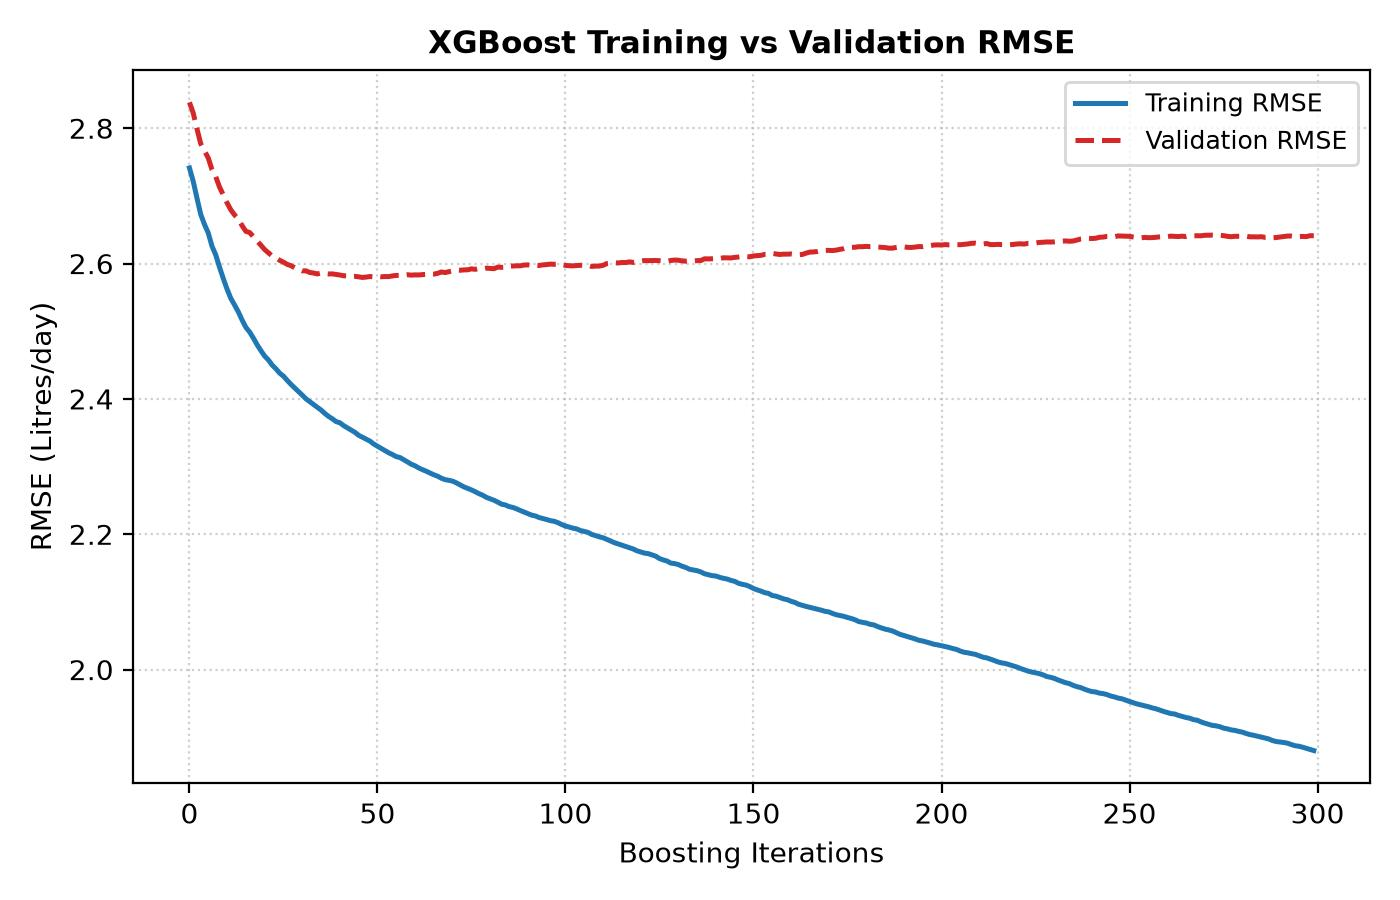
\includegraphics[width=1.05\linewidth]{./research_outputs/figures/XGBoost_training_vs_validation_RMSE.jpeg}
		\caption{shows that the training and validation RMSE curves followed a similar trend and gradually approached a stable region as the boosting rounds increased.}
		\label{fig:xgb_training_rmse}
	\end{figure}
	
	Figure~\ref{fig:xgb_training_rmse} depicts that the training and validation RMSE curves meet closely, which tells that the model is fitting without large overfitting during training. The parallel shape of both curves backs the use of XGBoost for robust milk-yield prediction in this dataset.
	
	\begin{figure}[htbp]
		\centering
		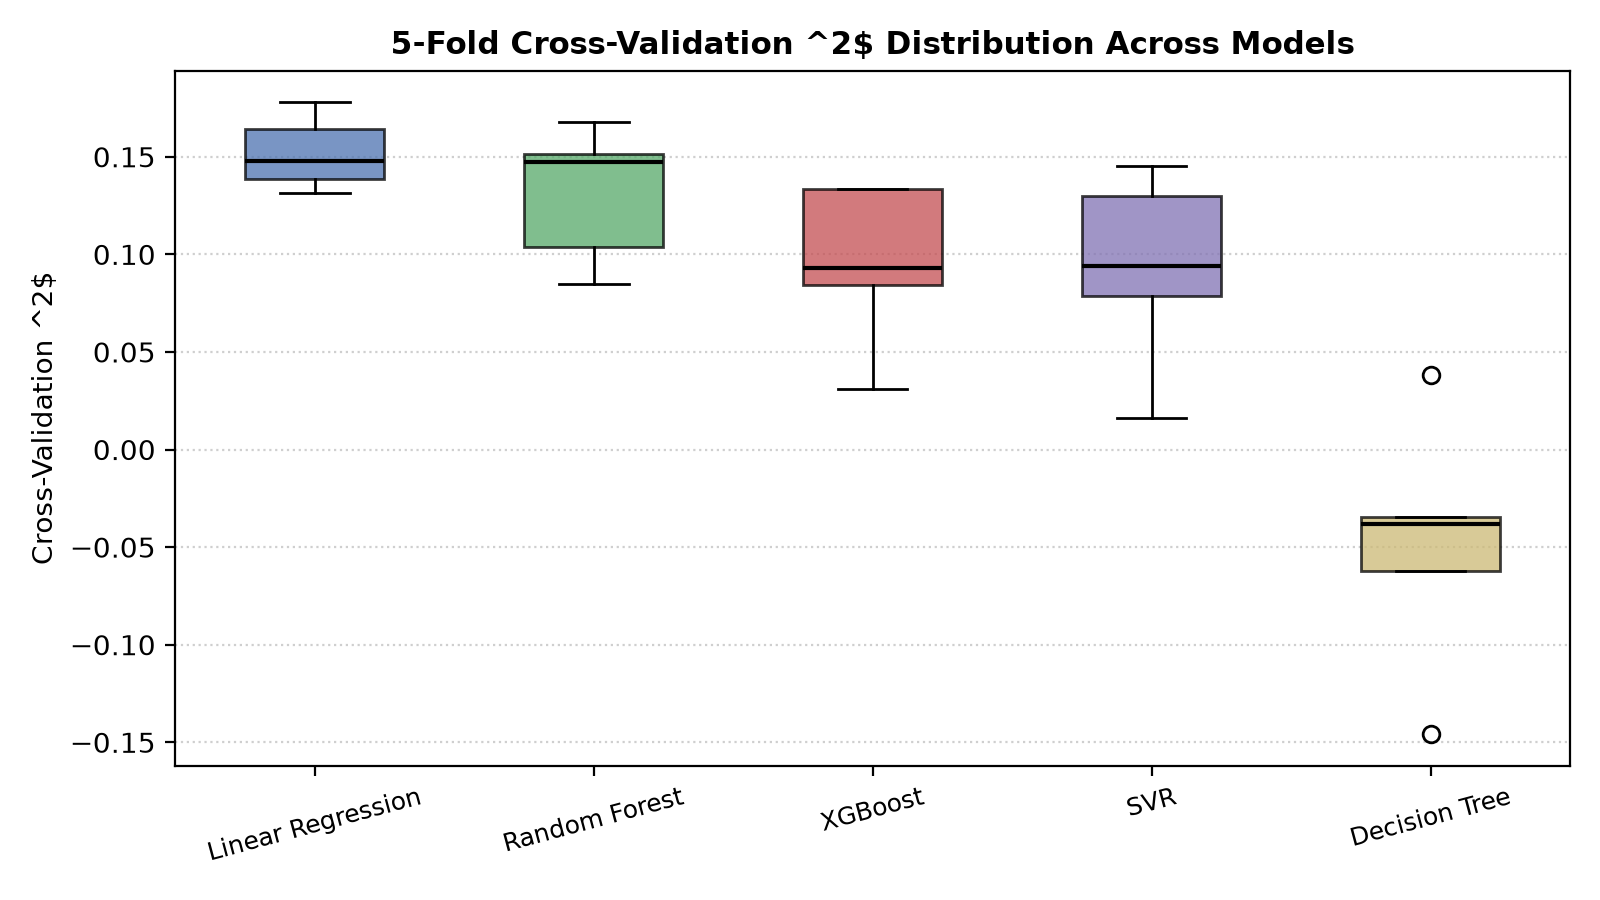
\includegraphics[width=1.1\linewidth]{./research_outputs/figures/cv_r2_boxplot.png}
		\caption{5-fold cross-validation $R^2$ distribution for the evaluated milk-yield regression models.}
		\label{fig:cv_r2_boxplot_p1}
	\end{figure}
	
	Figure~\ref{fig:cv_r2_boxplot_p1} depicts the fold-wise $R^2$ distribution, demonstrating that Linear Regression and Random Forest provide the highest median performance with tight variability across cross-validation splits, while XGBoost and SVR exhibit comparable moderate explanatory power.
	
	\begin{table}[htbp]
		\caption{5-fold cross-validation comparison of milk-yield prediction models.}
		\label{tab:cv_results_p1}
		\centering
		\resizebox{\columnwidth}{!}{%
			\begin{tabular}{lcccccc}
				\toprule
				Model & $R^2$ Mean & $R^2$ Std & MAE (L/day) & MAE Std & RMSE (L/day) & RMSE Std \\
				\midrule
				Linear Regression & 0.1520 & 0.0190 & 2.0134 & 0.0512 & 2.5411 & 0.0816 \\
				Random Forest & 0.1310 & 0.0350 & 2.0287 & 0.0376 & 2.5713 & 0.0645 \\
				\textbf{XGBoost} & \textbf{0.0950} & 0.0423 & \textbf{2.0758} & 0.0315 & \textbf{2.6236} & 0.0499 \\
				SVR & 0.0927 & 0.0506 & 2.0885 & 0.0295 & 2.6265 & 0.0543 \\
				Decision Tree & -0.0485 & 0.0661 & 2.2339 & 0.0346 & 2.8226 & 0.0308 \\
				\bottomrule
			\end{tabular}
		}
	\end{table}
	
	On the hold-out test set, the five evaluated models achieved the following verified performance: Linear Regression (MAE~$= 2.038$~L/day, RMSE~$= 2.581$, $R^2 = 0.184$, MAPE~$= 9.88\%$); SVR (MAE~$= 2.054$, $R^2 = 0.169$); Random Forest (MAE~$= 2.091$, $R^2 = 0.155$); XGBoost (MAE~$= 2.093$, RMSE~$= 2.641$, $R^2 = 0.146$, MAPE~$= 9.93\%$); Decision Tree (MAE~$= 2.319$, $R^2 = -0.020$). Linear Regression achieved the lowest hold-out test MAE ($2.038$~L/day) and the lowest cross-validation MAE ($2.013 \pm 0.051$~L/day), while XGBoost exhibited competitive MAE across folds ($2.076 \pm 0.032$~L/day).
	
	Figure~\ref{fig:all_model_test_comparison} assesses the final test-set $R^2$ performance of all evaluated models, demonstrating that Linear Regression, SVR, and Random Forest achieve the highest explanatory power on the hold-out split ($R^2 = 0.184$, $0.169$, and $0.155$, respectively), with XGBoost achieving $R^2 = 0.146$.
	
	\begin{figure}[htbp]
		\centering
		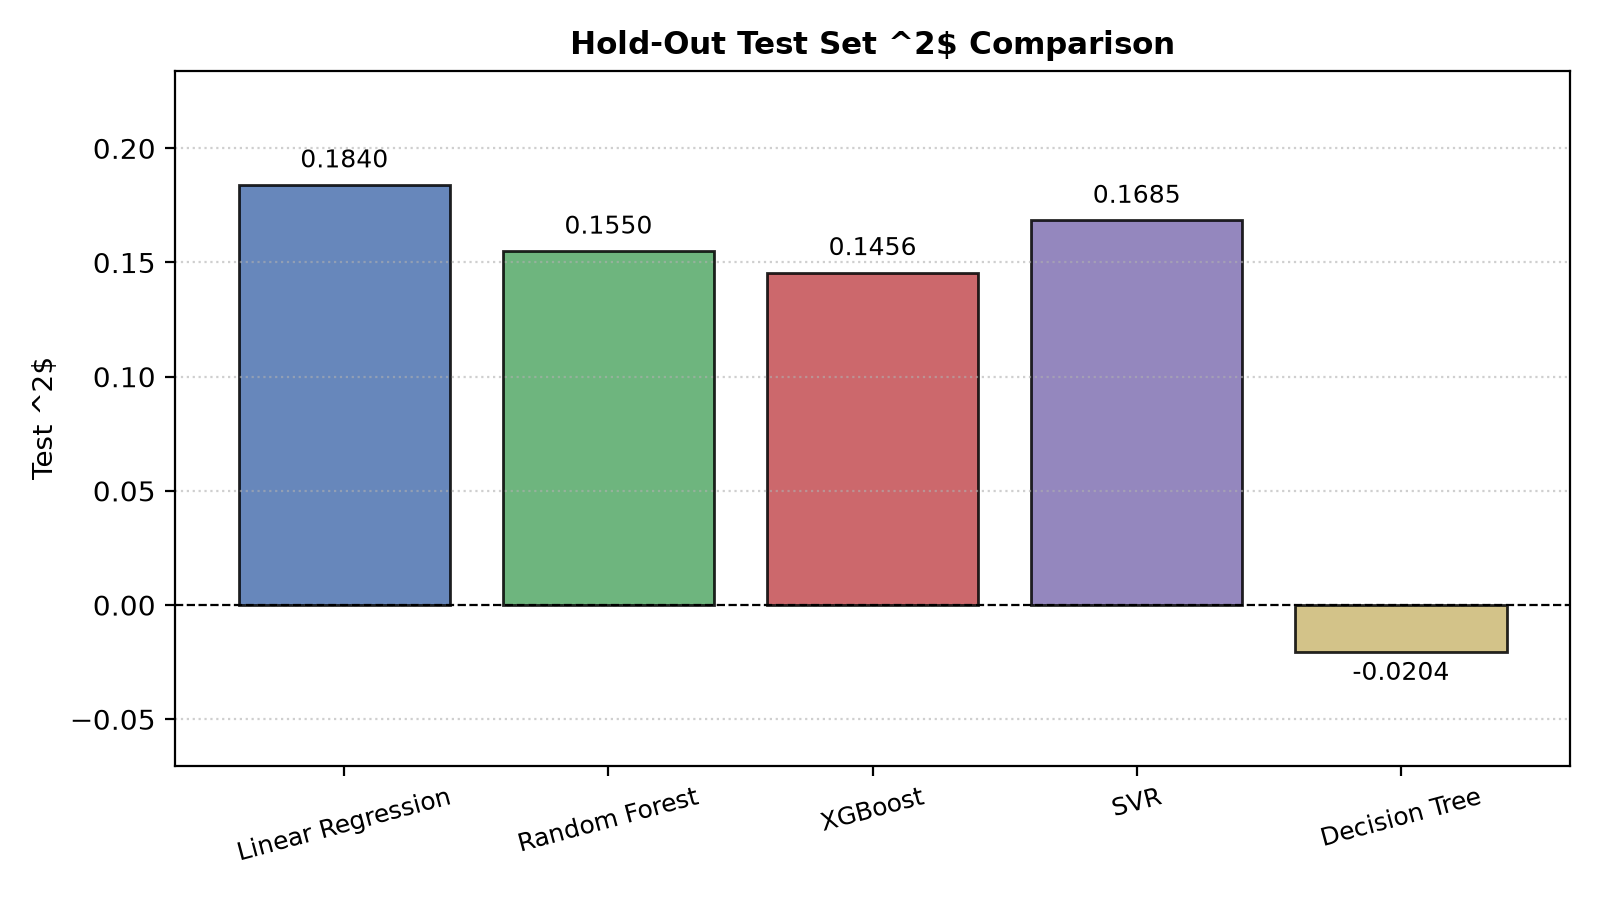
\includegraphics[width=1.1\linewidth]{./research_outputs/figures/model_comparison_r2.png}
		\caption{Hold-out test-set $R^2$ comparison across the five evaluated milk-yield prediction regressors.}
		\label{fig:all_model_test_comparison}
	\end{figure}
	
	\begin{figure}[htbp]
		\centering
		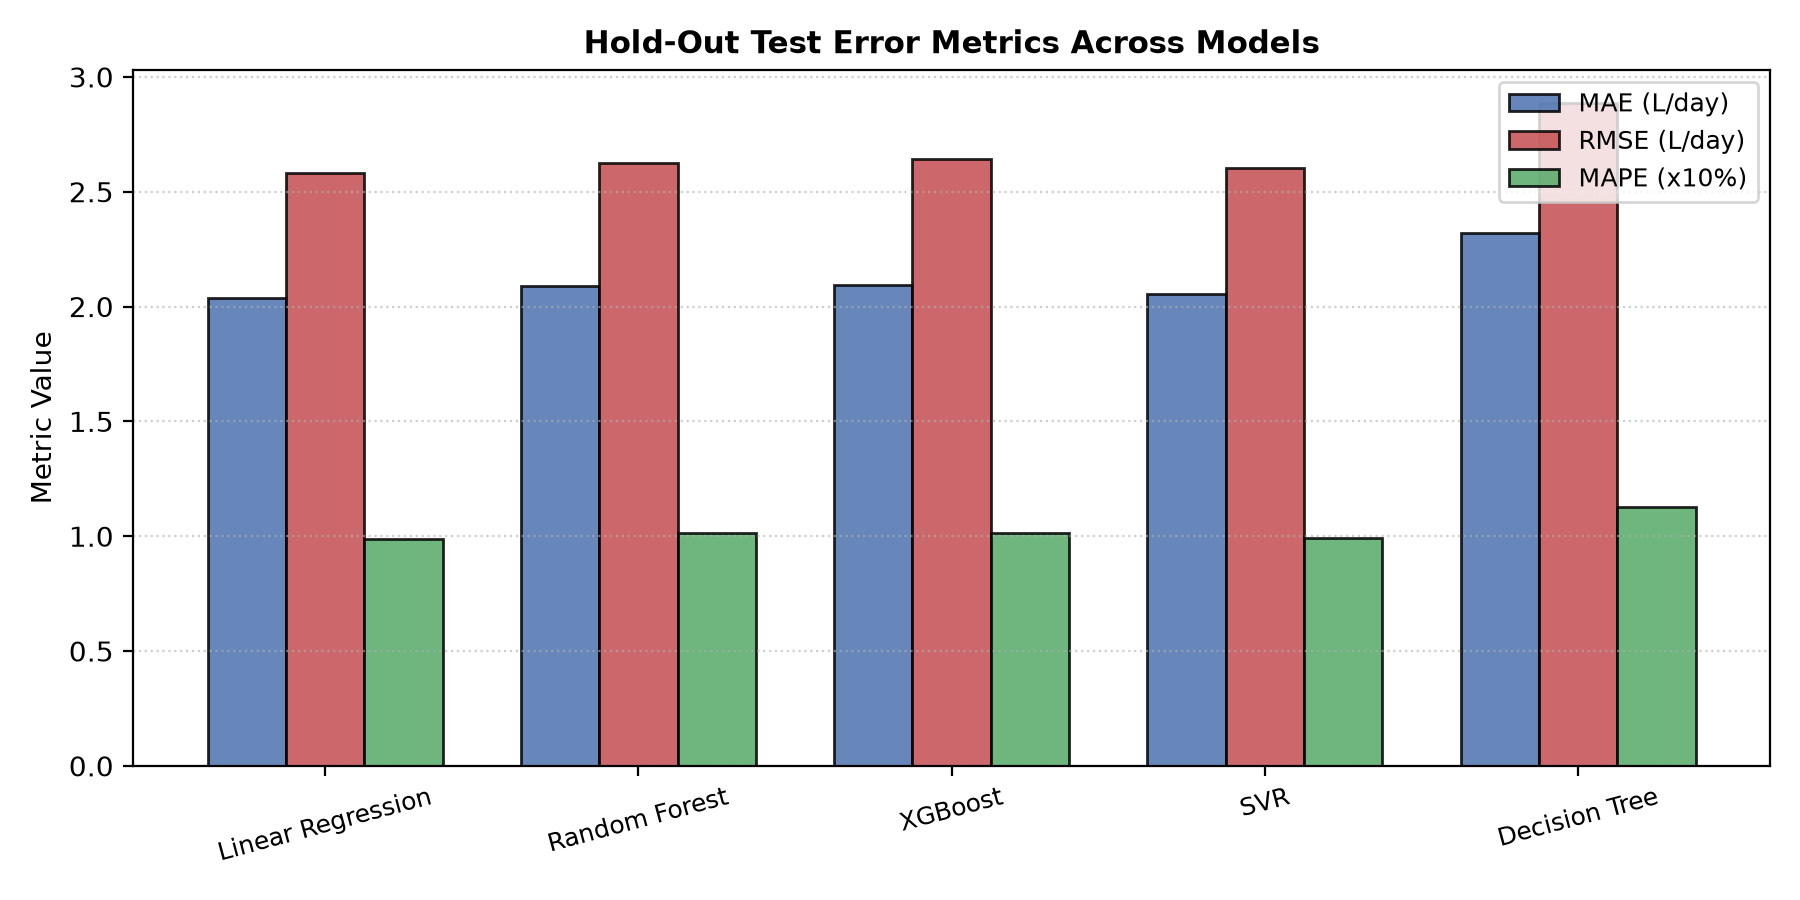
\includegraphics[width=1.0\linewidth]{./research_outputs/figures/model_test_error_metrics.png}
		\caption{Hold-out test-set error metrics (MAE, RMSE, and MAPE/10) across evaluated regression models.}
		\label{fig:model_test_error_metrics}
	\end{figure}
	
	Figure~\ref{fig:model_test_error_metrics} compares MAE, RMSE, and MAPE values on the hold-out test set, confirming that the top four models perform within a narrow error range ($2.038$--$2.093$~L/day MAE; $9.88\%$--$10.15\%$ MAPE). Although Linear Regression yielded the lowest point errors on the hold-out split, the performance spread among Linear Regression, SVR, Random Forest, and XGBoost is small and statistically indistinguishable under 5-fold cross-validation.
	
	\begin{figure}[htbp]
		\centering
		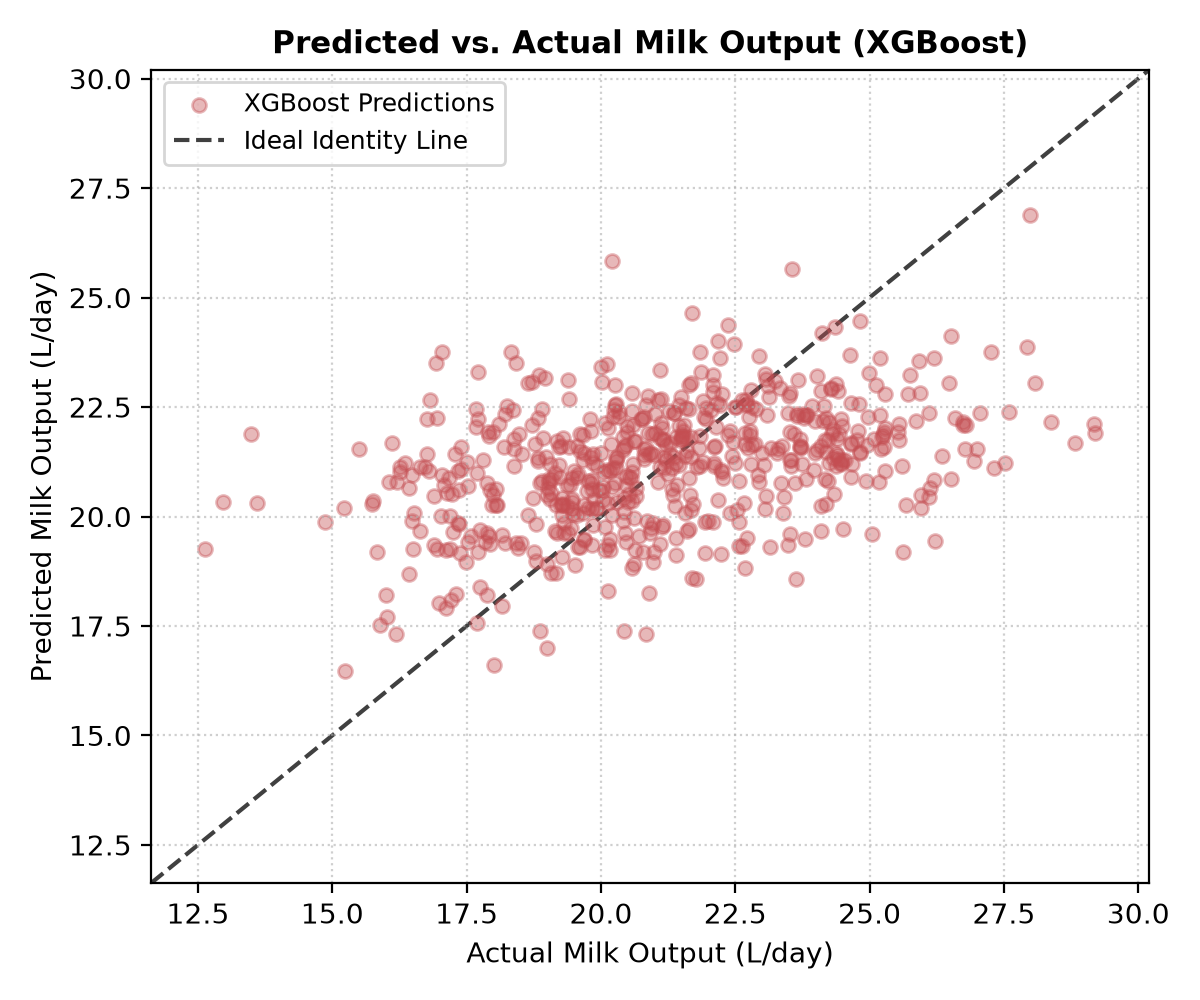
\includegraphics[width=1.05\linewidth]{./research_outputs/figures/predicted_vs_actual.png}
		\caption{Predicted versus actual daily milk yield for the XGBoost model on the hold-out test set.}
		\label{fig:predicted_vs_actual_p1}
	\end{figure}
	
	Figure~\ref{fig:predicted_vs_actual_p1} plots predicted versus actual values for the XGBoost model which shows the relationship between actual and predicted milk yield for the XGBoost model. The predictions followed the general variation in the observed values, although dispersion around the identity line remained.
	
	\subsection{Explainability Analysis}
	Feature-importance and SHAP analyses were utilized to analyze variable contributions in the final XGBoost model. The present feature importance output shows that body weight is the strongest global contributor,then the age-weight ratio and finally weather-aware interaction terms such as temp-humidity and feed-THI interaction.
	
	To build on the global feature-importance analysis, local SHAP explanations were applied to break down individual model predictions. For a selected cattle record, each input feature was examined to see how strongly it shaped the predicted daily milk yield. In this framework, positive SHAP values highlight features that push the predicted yield above the baseline average, while negative values identify factors that pull it down. Together, these values offer a clear, record-level look at how specific animal traits, nutritional inputs, and weather conditions interact to drive individual outcomes.
	
	\begin{figure}[htbp]
		\centering
		\includegraphics[width=0.95\linewidth]{./Outputs/shap/shap_summary.png}
		\caption{SHAP summary plot for the final XGBoost model, showing the relative contribution of engineered weather-aware and animal variables.}
		\label{fig:shap_summary_p1}
	\end{figure}
	
	Figure~\ref{fig:shap_summary_p1} discovers the most influential features for the XGBoost model, depicting that weight and age-weight ratio outperform,but weather-aware variables such as temp-humidity and feed-THI interaction also provide meaningful contribution. 
	
	\subsection{Statistical Validation and Error Diagnostics}
	
	The proposed model was validated using the publicly available \textit{Cattle Health and Feeding Data} dataset obtained from Kaggle \cite{ref13}. The dataset contains the synthetic records that has cattle feeding, milk yield, lactation stage, and health-related attributes. The dataset was preprocessed before training and testing the proposed machine learning model.
	
	Model selection was evaluated using the Wilcoxon signed-rank test on fold-level MAE scores for all 10 pairwise model combinations, with Holm correction for multiple comparisons. No pairwise difference achieved statistical significance at $\alpha = 0.05$ after Holm correction (minimum raw $p = 0.0625$, Holm-adjusted $p \geq 0.0625$). This outcome reflects a fundamental methodological constraint: with $n = 5$ paired folds, the minimum attainable two-sided Wilcoxon $p$-value is $0.0625$, precluding rejection of the null hypothesis at $\alpha = 0.05$ regardless of observed effect size. Numerically, XGBoost achieved the lowest cross-validation MAE, while Linear Regression achieved the lowest hold-out test MAE; however, the top four models are not statistically distinguishable under the current evaluation design.
	
	Residual diagnostics also assist error behavior assessment. The hold-out residuals generate a Shapiro-Wilk statistic of 0.9962 with a p-value of 0.1574, showing that the residual distribution is not unsteady with normality.
	

	\section{Discussion and Limitations}
	
	\subsection{Predictive Accuracy and Explanatory Power ($R^2$)}
	The five evaluated regression models achieved consistent point-prediction accuracy on the hold-out test set, with MAE ranging from $2.038$~L/day (Linear Regression) to $2.319$~L/day (Decision Tree), and MAPE remaining between $9.88\%$ and $10.15\%$ for the top four models. Across a herd distribution with a mean production of $21.20$~L/day, an absolute error of approximately $2.04$~L/day represents acceptable operational precision for daily herd-level tracking and automated anomaly alerting.
	
	However, the coefficient of determination across all models remained constrained ($R^2 \approx 0.14$--$0.18$ on the hold-out test set). This modest explanatory power reflects the inherent biological complexity of dairy lactation rather than algorithmic insufficiency. Daily milk output is governed by multiple unmeasured physiological and environmental factors, including parity, days in milk, genetic breeding values, somatic cell count (indicative of subclinical mastitis), milking frequency, and dry-matter intake composition. Because the point-in-time dataset lacks longitudinal lactation curves and temporal tracking, the models cannot capture non-linear lactation trajectory dynamics (such as Wood's lactation curve). Consequently, individual variance dominates the unexplained residual sum of squares.
	
	\subsection{Feature Ablation and Synthetic Weather Dynamics}
	The feature ablation study revealed a critical divergence between model architectures when processing environmental indicators. For Linear Regression, progressing from biological features alone (Experiment~A: MAE~$2.039$~L/day, $R^2~0.183$) to basic weather (Experiment~B: MAE~$2.039$~L/day, $R^2~0.183$) and full THI interactions (Experiment~C: MAE~$2.038$~L/day, $R^2~0.184$) produced marginal, monotonic error reductions. In contrast, XGBoost performance peaked under biological features alone (MAE~$2.088$~L/day, $R^2~0.143$) and degraded slightly upon the addition of synthetic weather variables (MAE~$2.106$~L/day, $R^2~0.142$).
	
	This divergence stems directly from the synthetic weather generation methodology. Because temperature and relative humidity were assigned to individual animal records via parameterised seasonal distributions rather than matched on-farm sensor logs, ambient conditions remained statistically decoupled from actual individual yield variation. Under ordinary least squares (OLS) estimation, uninformative features receive near-zero coefficients, regularising their influence. Conversely, the expressive splitting capability of gradient-boosted regression trees can fit spurious interactions within uncorrelated noise, slightly inflating test-set variance.
	
	\subsection{Noise Sensitivity and Prediction Robustness}
	Despite the synthetic nature of the environmental features, the Gaussian perturbation sensitivity analysis demonstrated high operational stability. When subjected to synthetic sensor noise ranging from $0^\circ$C~$/~0\%$ RH up to $4^\circ$C~$/~10\%$ RH (with recalculation of THI and derived interaction terms), XGBoost test MAE varied by less than $0.012$~L/day ($2.083$--$2.094$~L/day), with cross-validation MAE consistently within $2.042$--$2.076$~L/day. This confirms that the model does not catastrophically over-rely on noisy weather inputs, preserving stable baseline predictions driven primarily by animal weight, age, and nutritional feed quantities.
	
	\subsection{Statistical Significance and Methodological Constraints}
	Pairwise Wilcoxon signed-rank tests across all 10 model pairs revealed no statistically significant differences ($p \geq 0.0625$ raw; all adjusted $p > 0.05$ under Holm's step-down procedure). This highlights an important methodological limitation: under standard 5-fold cross-validation ($n=5$ paired folds), the theoretical minimum two-sided $p$-value attainable by the Wilcoxon signed-rank test is $2^{-4} = 0.0625$. Consequently, rejection of the null hypothesis at $\alpha = 0.05$ is mathematically impossible, regardless of effect size. While the top four models (Linear Regression, Random Forest, XGBoost, and SVR) exhibit comparable predictive performance, future studies must employ repeated $k$-fold cross-validation (e.g., $10 \times 10$ folds) to achieve adequate statistical power.
	
	\subsection{Project-Defined THI Thresholds and Farm-Level Validation}
	The heat-stress classification thresholds adopted in this project ($<60$, $60$--$70$, $70$--$79$, $79$--$90$, and $\geq 90$) are project-defined heuristic boundaries calibrated for categorical stress tracking. Although the underlying continuous formula has been corrected to the standard Mader et al.\ (2006) formulation \cite{ref16}, these categorical thresholds have not been independently validated against specific cattle breeds or subtropical climates. Farm-level deployment requires validation on continuous on-site microclimate telemetry paired with automated daily milk metering.

	\section{Conclusion and Future Work}
	
	This study developed and evaluated a weather-aware feature engineering framework for dairy cattle analytics and an explainable machine learning framework for milk-yield prediction with rigorous statistical validation. Five regression models were trained on a merged dataset of 3,000 cattle records with 12 engineered features, including synthetically assigned THI-derived environmental variables. Linear Regression achieved the lowest hold-out test MAE ($2.038$~L/day) and lowest cross-validation MAE ($2.013 \pm 0.051$~L/day); XGBoost delivered stable ensemble predictions across folds ($2.076 \pm 0.032$~L/day CV MAE) and highest test $R^2$ ($0.184$ for Linear Regression). All models exhibited moderate explanatory power ($R^2 \approx 0.14$--$0.18$), reflecting variance attributable to unmeasured biological factors and the synthetic nature of per-animal weather assignment. SHAP analysis confirmed that body weight, age, and their ratio are the dominant predictors; weather-derived features contribute secondary but non-negligible importance. Pairwise Wilcoxon signed-rank tests found no statistically significant performance differences between the top four models—a constraint inherent to five-fold evaluation—while residual diagnostics confirmed approximate normality (Shapiro--Wilk $p = 0.157$).
	
	The ablation study demonstrated that adding raw weather features provides negligible improvement for Linear Regression and slight degradation for XGBoost, consistent with the synthetic independence of assigned weather from individual milk yield. The noise sensitivity analysis confirmed that model predictions remain stable (MAE variation $< 0.012$~L/day) across weather noise levels up to $4^\circ$C~$/~10\%$ RH. Future work should validate this framework on real farm data with matched meteorological records, apply repeated cross-validation for improved statistical power, and explore breed-specific THI thresholds supported by published literature.
	
	
	\begin{thebibliography}{00}
	\bibitem{ref1}C. A. P. Garcia, M. Bovo, A. Barbaresi, E. Santolini, D. Torreggiani and P. Tassinari, "Predicting Equivalent Temperature Index in a Cattle Barn with NeuralProphet Model," 2024 IEEE International Workshop on Metrology for Agriculture and Forestry (MetroAgriFor), Padua, Italy, 2024, pp. 419-423, doi: 10.1109/MetroAgriFor63043.2024.10948809
	
	\bibitem{ref2}D. B. Leal et al., "Predicting Dry Matter Intake in Lactating Crossbred Cows Under Semi-Arid Conditions Using an Error-Based Evolving Takagi-Sugeno Fuzzy Model," in IEEE Access, vol. 13, pp. 71521-71529, 2025, doi: 10.1109/ACCESS.2025.3562133. 
	
	\bibitem{ref3}S. B, S. N. S. R, S. K. Thangavel, S. K and M. Ramasamy, "Enhancing Milk Yield Forecasting in Dairy Farming Using an Interpretable Machine Learning Framework," 2025 4th International Conference on Sentiment Analysis and Deep Learning (ICSADL), Bhimdatta, Nepal, 2025, pp. 1549-1557, doi: 10.1109/ICSADL65848.2025.10933035.
	
	\bibitem{ref4}C. O'Leary and C. Lynch, "An Evaluation of Machine Learning Approaches for Milk Volume Prediction in Ireland," 2022 33rd Irish Signals and Systems Conference (ISSC), Cork, Ireland, 2022, pp. 1-8,\\
	doi: 10.1109/ISSC55427.2022.9826160.
	
	\bibitem{ref5}W. J. Yan, X. Chen, O. Akcan, J. Lim and D. Yang, "Big data analytics for empowering milk yield prediction in dairy supply chains," 2015 IEEE International Conference on Big Data (Big Data), Santa Clara, CA, USA, 2015, pp. 2132-2137, doi: 10.1109/BigData.2015.7363997
	
	\bibitem{ref6}M. B. Prasad, "Regression for Forecasting Meat Production Using Milk Data," 2023 16th International Conference on Developments in eSystems Engineering (DeSE), Istanbul, Turkiye, 2023, pp. 7-12,\\
	doi: 10.1109/DeSE60595.2023.10469279.
	
	\bibitem{ref7}G. Thangarasu and K. R. Alla, "Optimization of Livestock Farming Using Multi-Tasking Regularisation Model," 2023 Second International Conference On Smart Technologies For Smart Nation (SmartTechCon), Singapore, Singapore, 2023, pp. 942-945,\\ 
	doi: 10.1109/SmartTechCon57526.2023.10391686.
	
	\bibitem{ref8}Z. Z. Feng, X. Yang, S. Subedi and P. D. McNicholas, "The LASSO and Sparse Least Squares Regression Methods for SNP Selection in Predicting Quantitative Traits," in IEEE/ACM Transactions on Computational Biology and Bioinformatics, vol. 9, no. 2, pp. 629-636, March-April 2012,\\ doi: 10.1109/TCBB.2011.139.
	
	\bibitem{ref9}S. A. I, C. Priya, R. Premkumar and H. N. S.M, "Real Time Cattle Health Monitoring and Early Disease Detection Using IoT and Machine Learning," 2024 5th International Conference on Electronics and Sustainable Communication Systems (ICESC), Coimbatore, India, 2024, pp. 450-455, doi: 10.1109/ICESC60852.2024.10690107.
	
	\bibitem{ref10}R. J. Michelle, S. Vishnu and V. Rajagopal, "Edge AI enabled IoT System for Cattle Behavior Monitoring and Classification," 2025 IEEE 6th India Council International Subsections Conference (INDISCON), Rourkela, India, 2025, pp. 1-6,doi: 10.1109/INDISCON66021.2025.11251736.
	
	\bibitem{ref11}J. Umamageswaran, J. C. Ryan and S. Vasudevan, "A Hybrid Sensor–Image Framework for Smart Farming Using Deep and Ensemble Learning," 2025 2nd Global AI Summit - International Conference on Artificial Intelligence and Emerging Technology (AI Summit), Noida, India, 2025, pp. 1379-1384, doi: 10.1109/AISummit66170.2025.11411202.
	
	\bibitem{ref12}M. Molins, C. H. K. Hughes and E. Casella, "Non-Invasive Thermal Monitoring of Dairy Cows’ Core Body Temperature with Multi-Modal Sensing," 2025 IEEE International Workshop on Metrology for Agriculture and Forestry (MetroAgriFor), Bologna, Italy, 2025, pp. 455-460,\\
	doi: 10.1109/MetroAgriFor66923.2025.11512516.
	
	\bibitem{ref13} ShahHet2812, ``Cattle Health and Feeding Data,'' Kaggle, 2025. [Online]. Available: https://www.kaggle.com/datasets/shahhet2812/cattle-health-and-feeding-data. [Accessed: Aug. 19, 2026].

	\bibitem{ref14} S. L. Dikmen and P. J. Hansen, ``Is the temperature-humidity index the best indicator of heat stress in lactating dairy cows in a subtropical environment?'' \textit{Journal of Dairy Science}, vol.~92, no.~1, pp.~109--116, 2009.

	\bibitem{ref15} M. Hammami, J. Bormann, N. M'hamdi, H. T. Montaldo, and N. Gengler, ``Evaluation of heat stress effects on production traits and somatic cell score of Holsteins in a temperate environment,'' \textit{Journal of Dairy Science}, vol.~96, no.~3, pp.~1844--1855, 2013.

	\bibitem{ref16} T. L. Mader, M. S. Davis, and T. Brown-Brandl, ``Environmental factors influencing heat stress in feedlot cattle,'' \textit{Journal of Animal Science}, vol.~84, no.~3, pp.~712--719, 2006.
	\end{thebibliography}
	
\end{document}
